\section{A*mbush}

In this section we propose \ambush, an $A^*$-based
algorithm that solves the ambush generation problem. 
It consists in a modification of $g$ function, that favours
path diversity. We will call this function $g'$.

Let $\Psi(v,i) = 1+(\# j : j \in A \wedge v \in path(j))$,
be the number of agents different from agent $i$, that have the 
node $v$ in their paths towards $t$ plus one. If an agent is not trying to 
reach node $t$ at the moment, or it has not performed the 
search for the node yet, it's path counts as empty. 
Therefore, the agent is not taken into account when calculating
$\Psi(v,i)$'s value. 

It is considered that $g'(pos(i),i) = 0$ for the initial node.
 Let $<v,w>$ be the next edge that should be expanded
from the node $v$, in any of the algorithm's iterations. In
these conditions, the expression that determines $g'$'s value
is $g'(w, i) = g'(v,i) + \lambda_i(<v,w>) \cdot \Psi(w,i)^2$.

Given that $\Psi(v,i) \geq 1$, the path determined by $A^*mbush$
is optimal under the new definition of $g'$. Hence, the properties of
 $A^*$ are preserved \cite{art2}. Nevertheless the path might not 
 be optimal for the original costs function $g$.

Note that $\Psi(v,i) = 1$ for every node $v$ that is not considered
in the path of any agent different to $i$. Similarly,
$\Psi(v,i) > 1$ in any other case. This condition allows the 
agents to consider exploring sub-optimal paths in the 
original graph. The less agents explore this routes, the greater
the chance given to other agents to travel trough them.

\subsection{Complexity}

It is possible to precompute the
function $\Psi$ for node cost's increment. If this function is stored
in a constant structure with fast access, the cost of calculating
$g'$ becomes equal to the cost of computing $g$.
Therefore, the only change if the algorithm's cost
 lays in the initial calculation of function $\Psi$.

The asymptotic complexity of $A^*mbush$ is:
$\bigO(|V|log(|V|) + |V|*h + |E| + |A|*|V| )$.

In the field of video games, the graphs of interest are
given by the polygonal division scheme of the map
\cite{book3,art1} (this polygons tend to have a small
amount of sides), according to the traversable regions 
and their respective adjacencies \cite{book3,art1}. 
Since the number of sides for the polygons is small, this 
graphs tend to have little density. In consequence,
$|E| \in \bigO(|V|)$, this means that the execution 
time of this methods for the graphs of interest in the
area of video games, is considered to be
$\bigO(|V|(log(|V|) + h + |A|) )$. 
The amortized cost of the increment function is $\bigO(|V|)$,
therefore, the amortized cost of the A$^*$mbush algorithm
equals the A$^*$ cost.

\begin{comment}
Figure
\ref{fig:graph_decomp} shows a clear example of a map 
broken into polygons. Each one of them is considered to
be a node in the search space. Two nodes are adjacent if 
their polygons share a common side. 

\begin{figure}[htp]
\centerline{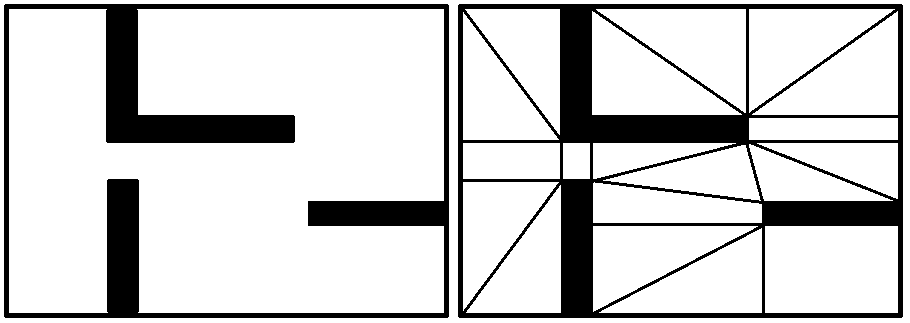
\includegraphics[width=0.6\columnwidth]{figures/graph_decomposition.png}}
\caption{Up: Game map, the black blocks are the obstacles
              Down: Decomposition of the map into convex polygons}
\label{fig:graph_decomp}
\end{figure}
\end{comment}

